\documentclass[a4paper]{report}

\usepackage[utf8]{vietnam}
\usepackage[left=1.5cm,right=1cm,top=1.5cm,bottom=1.5cm]{geometry}
\usepackage{amsmath, amsthm, amssymb,verbatim}
\usepackage{tikz}
\usetikzlibrary{calc,angles,quotes,arrows,decorations.markings}

\tikzset{
	ex_markstyle/.style={},
	ex_mark/.style  n args={1}{decoration={ markings, %
			mark= at position 0.5 with
			with{
				\ifnum#1=1
				\draw[ex_markstyle] (0pt,-2pt) -- (0pt,2pt);
				\fi
				\ifnum#1=2
				\draw[ex_markstyle] (-1pt,-2pt) -- (-1pt,2pt);
				\draw[ex_markstyle] (1pt,-2pt) -- (1pt,2pt);
				\fi
				\ifnum#1=3
				\draw[ex_markstyle] (-2pt,-2pt) -- (-2pt,2pt);
				\draw[ex_markstyle] (0pt,-2pt) -- (0pt,2pt);
				\draw[ex_markstyle] (2pt,-2pt) -- (2pt,2pt);
				\fi
				\ifnum#1=4
				\draw[ex_markstyle] (-1pt,-1pt) -- (1pt,1pt);
				\draw[ex_markstyle] (-1pt,1pt) -- (1pt,-1pt);
				\fi
		} },
		pic actions/.append code=\tikzset{postaction=decorate}},
}

\begin{document}
	\chapter*{ĐÁNH DẤU GÓC BẰNG TIKZ 3.1}
	\section{Góc thường}
	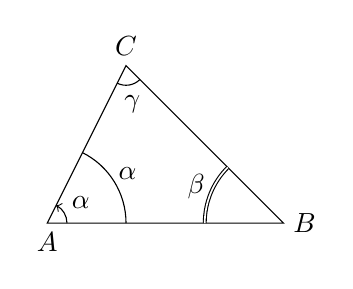
\begin{tikzpicture}
		\path (0,0) coordinate (A)node[below]{$A$}
		(3,0) coordinate (B)node[right]{$B$}
		(1,2) coordinate (C)node[above]{$C$};
		\draw (B)--(A)--(C)--cycle;
		\pic["$\alpha$", draw=black, angle eccentricity=1.2, angle radius=1cm]
		{angle=B--A--C}; %góc
		\pic["$\beta$", draw=black, double, angle eccentricity=1.2, angle radius=1cm]
		{angle=C--B--A}; %góc double
		\pic["$\gamma$", draw=black, mark=|, angle eccentricity=2, angle radius=0.25cm]
		{angle=A--C--B}; %góc
		\pic["$\alpha$", draw=black, ->, angle eccentricity=2, angle radius=0.25cm]
		{angle=B--A--C}; %Mũi tên
	\end{tikzpicture}
	\section{Góc vuông}
	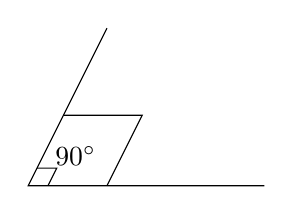
\begin{tikzpicture}
		\path (0,0) coordinate (A)
		(3,0) coordinate (B)
		(1,2) coordinate (C);
		\draw (B)--(A)--(C);
		\pic[draw=black, angle radius=1cm]
		{right angle=B--A--C}; %Góc vuông
		\pic["$90^{\circ}$", draw=black, angle eccentricity=2, angle radius=0.25cm]
		{right angle=B--A--C}; %Góc vuông
	\end{tikzpicture}
	\section{Đánh dấu góc bằng nhau}
	
	\begin{tikzpicture}[scale=1, font=\footnotesize, line join=round, line cap=round, >=stealth]
		\path 
		(1,3) coordinate (A)
		(0,0) coordinate (B)
		(4,0) coordinate (C)
		;
		
		\draw (A)--(B)--(C)--cycle;
		
		\foreach \p/\r in {A/90,B/-120,C/-60}
		\fill (\p) circle (1.5pt) node[shift={(\r:3mm)}]{$\p$};
		
		\pic[draw, angle radius=0.5cm, ex_mark=1,ex_markstyle/.style={scale=3}] {angle = B--A--C};
		
		\pic["$\alpha$",draw,angle radius=0.5cm,ex_mark=2] {angle = C--B--A};
		
		\pic[draw,angle radius=0.5cm,ex_mark=3] {angle = A--C--B};
	\end{tikzpicture}
	\begin{tikzpicture}[scale=1, font=\footnotesize, line join=round, line cap=round, >=stealth]
		\path 
		(1,3) coordinate (A)
		(0,0) coordinate (B)
		(4,0) coordinate (C)
		;
		
		\draw (A)--(B)--(C)--cycle;
		
		\foreach \p/\r in {A/90,B/-120,C/-60}
		\fill (\p) circle (1.5pt) node[shift={(\r:3mm)}]{$\p$};
		
		\pic[draw,ex_mark=1,,ex_markstyle/.style={scale=3}] {angle = B--A--C};
		
		\pic["$\alpha$",draw,angle radius=0.5cm,ex_mark=2] {angle = C--B--A};
		
		\pic[draw,angle radius=0.5cm,ex_mark=4,ex_markstyle/.style={scale=2}] {angle = A--C--B};
	\end{tikzpicture}
	\section{Tham khảo}
	\begin{enumerate}
		\item \verb|https://tikz.dev/library-angle|
		\item \verb|https://tex.stackexchange.com/questions/336244/various-questions-on-the-pic-command-from-the-tikz-angles-library|
		\item Hồ Hà Đặng \&\, Hoàng Hải
	\end{enumerate}
\end{document}